\documentclass[../thesis.tex]{subfiles}
\begin{document}
This chapter offers a comprehensive survey of the research relevant to this thesis. Our objectives are to establish the contextual backdrop of previous counting and clustering methods as well as to introduce the fundamentals of the tools we use in our work.
To achieve this, we present the two most significant architectures to this thesis, convolutional neural networks and transformers.
We then outline many of the foundational clustering methods as well as their limitations before discussing deep-learning-based improvements to them.
Finally, we delve into the recent advancements in the field of automated counting. We describe the task of class-specific counting and how its limitations prompted the advent of class-agnostic counting.
In describing the relevant work on class-agnostic counting, we make clear the motivation behind our work in this area.


\section{Network Architectures}
In this section, we discuss the two main architectures utilised in this dissertation and by others working in similar fields, namely convolutional neural networks and transformers.

\subsection{Convolutional Neural Networks}

Inspired by Neocognition \cite{fukushima1980neocognitron}, Convolutional Neural Networks (CNNs) were introduced and effectively trained using back-propagation \cite{lecun1989backpropagation, lecun1998gradient}. 
The early CNNs, known as LeNets \cite{lecun1989backpropagation}, were initially devised for the recognition of handwritten digits. 
These networks featured convolutional layers followed by sigmoid units to provide non-linearity, with average pooling layers. 
The networks were structured hierarchically,
with the initial layers being responsible for extracting local features from the input and the later layers gradually amalgamating them into more complex global features. 
The high-dimensional convolutional features are finally summarised using a fully connected layer to produce an image classification. 

CNNs are an example of parameter sharing. 
The learned feature extractors are applied across the whole input, which is more efficient and encourages the filters to learn to recognise general translation-invariant features.
Early networks were trained using a combination of the mean squared error (MSE) and maximum a posteriori (MAP) losses. 
While LeNets excelled on the MNIST dataset \cite{lecun1998gradient}, they encountered challenges when applied to real-world vision problems in the 1990s. 
Two primary obstacles emerged: first, training large-scale CNNs necessitated an impractical number of iterations to converge using stochastic gradient descent (SGD) due to limited computational resources at the time; second, despite spatial sharing of convolutional kernels, typical CNNs still required millions of parameters, rendering them susceptible to overfitting on datasets like MNIST.

The breakthrough for CNNs in computer vision was in 2012, with the advent of large-scale datasets and high-performance Graphics Processing Units (GPUs).
This, combined with a series of innovations in CNNs, rapidly improved their performance in computer vision applications.
AlexNets \cite{krizhevsky2012imagenet} employed rectified linear units (ReLUs) as their non-linear activations.
To decrease the resolution of their data, highlight the most distinctive features, and improve their spatial invariance, AlexNets also introduced max-pooling layers.
To combat overfitting, dropout \cite{srivastava2014dropout} and data augmentation techniques, including colour jittering and random cropping, are commonly incorporated during training. These augmentations disrupt the usual training of a network and create a more robust understanding of the true patterns in the images rather than of the exact images themselves. 

From 2014, significant improvements were made by adopting deeper architectures \cite{szegedy2015going,simonyan2014very}.
Many of the contemporary counting methods use Residual Networks (ResNets), which have not significantly changed since they were introduced in 2016 \cite{he2016resnet}.
These networks, often with over a hundred layers, leveraged skip connections, where the output of a layer is added to the output of later layers.
The incorporation of residual units facilitates more effective backpropagation of gradients. 

To achieve pixel-level predictions such as semantic segmentation \cite{He2017, Brabandere2017} or the density map regression used in many counting methods \cite{ranjan2021Famnet, shi2022represent, liu2022countr} rather than image-level classifications, CNNs often employ two stages: downsampling and upsampling.
The downsampling stage resembles the architecture of a classification network, summarising the data into a lower spatial resolution but higher dimensional, and so more informative, feature space.
The upsampling stage increases the spatial resolution of this condensed feature back to that of the original image.
This is achieved using either alternating upsampling and convolutional layers or `transposed' convolutional layers.
The training loss of these networks varies based on the task at hand but generally can be grouped into pixel-wise losses, such as pixel-wise mean squared error \cite{ranjan2021Famnet, shi2022represent}, or feature-wise \cite{johnson2016perceptual} or image-wise \cite{Goodfellow2014} perceptual losses.

CNNs, by their nature, find relationships between spatially local features, starting at a pixel level and gradually expanding their receptive field, the area of the input which affects a single feature in later layers. 
However, even with the increased receptive field of later layers, a deep feature is constructed hierarchically from features with smaller receptive fields leading to an understanding of the image that is by definition local-context-first.
While this locally aware approach is useful for tasks like image classification where the object of interest is spatially contiguous, we show it is not well suited for other tasks such as counting where spatially disparate objects are as important as close objects.

There have been various approaches to increasing the receptive field of a given feature or network, such as dilation \cite{li2018csrnet, bai2020adaptive} or multi-scale features \cite{ranjan2021Famnet}. 
In dilation, the weights of kernels are applied to samples which are no longer spatially adjacent, effectively introducing `holes' to the convolutional kernel. While dilation does increase the receptive field faster than non-dilated kernels, they are either still inherently local-first as they do not take global context into account directly or they are so dilated that they are no longer functional as convolutional kernels.
Multi-scale features are generally created by using a set of scaled versions of the input image or by combining features from different latent layers which have different spatial resolutions \cite{gao2019res2net,olimov2023consecutive}.


Instead of parameter sharing across spatial dimensions (a characteristic of CNNs in image processing), an alternative approach is parameter sharing across a temporal dimension. This concept underlies Recurrent Neural Networks (RNNs), which were originally developed in 1986 by \citet{rumelhart1986learning} and which are most commonly used for text processing or generation.
Each feature neuron in an RNN takes the output from the previous time steps as its input. 
While this arrangement endows RNNs with a basic form of memory, it also exacerbates issues related to vanishing and exploding gradients. The root cause of this problem lies in the repeated multiplication of parameter values during gradient computation, leading to gradient explosions when parameters exceed 1 or gradients vanishing when parameters fall below 1.

Long Short-Term Memory (LSTM) networks, introduced by \citet{hochreiter1997long} in 1997, try to mitigate the amnesia caused by these gradient-related challenges. LSTMs incorporate input, output, and forget gates within each recurrent cell. These gates enable the network to determine when to update information within the cell and when to discard it rather than relying on the same parameter multiplication at every time step. 
In the case of RNNs, which process words sequentially, they consider the present word and other words from the past within a defined `context window'. As a consequence, more recent words near the end of a sentence receive greater attention, while earlier words gradually get lost to volatile neural activations.

The introduction of the \textit{attention} mechanism revolutionised the text processing paradigm by providing all words in a sequence equal access to all other parts of the sequence, concurrently and in a parallel fashion. 
This eliminates the time-consuming aspect of serial processing and also combats the amnesia of RNNs and LSTMs. Initially, the attention mechanism was integrated into sequential RNNs for language translation systems \cite{bahdanau2016neural}. However, as the field evolved, developments in Transformer-based large language models dispensed with RNNs altogether and relied exclusively on the highly efficient parallel Attention scheme; 
this is further discussed in \Cref{LTCA__sec__lit_rev__transformers}.
Counting, as we see it, requires an understanding of features that may appear far from each other to gain an informed representation of the objects present.
As such, the global-context-aware features generated by utilising attention mechanisms appear well suited to the task of counting. Due to this intrinsic capability, we utilise them in \Cref{sec__LTCA,,sec__ABC123}.




\subsection{Attention and Vision Transformers.}\label{LTCA__sec__lit_rev__transformers}
Attention layers vary from convolutional or recurrent layers as they dynamically adjust the weighting of input values rather than using static weights for all sections of the input data. 
An attention layer operates on three main components, namely the queries, $Q$, the keys, $K$, and the values, $V$, in three base steps: alignment scores, weights, and context vectors.

Alignment scores are found between each query, $q$, and each key $k_i$:
\begin{equation}\label{LTCA__eq__attention_alignment_score}
    z_{\vec{q},\vec{k_i}}=\vec{q} \cdot \vec{k_i} 
\end{equation}
\myequations{Alignment Score}
These alignment scores are then used to find weights using a softmax:
\begin{equation}\label{LTCA__eq__attention_weight_calc}
    \alpha_{\vec{q},\vec{k_i}}=\text{softmax}(z_{\vec{q},\vec{k_i}}) = \sigma(\vec{z})_{i} =\frac{e^{z_{\vec{q},\vec{k_i}}}}{\sum_{j=1}^{\vec{K}} e^{z_{\vec{q},\vec{k_j}}}}
\end{equation}
\myequations{Weights Score}
The weights are then used to find a context vector from the value vectors $\vec{v}_{\vec{k_i}}$: 
\begin{equation}
    \text{attention}(\vec{q}, \vec{K}, \vec{V}) = \sum_i \alpha_{\vec{q},\vec{k_i}} \vec{v}_{\vec{k_i}}
\end{equation}
\myequations{Attention Vector}
Transformers proposed by \citet{vaswani2017attention} use this multiplicative attention as it is more efficient  than the initially proposed additive attention. They also employ only attention layers instead of combinations of attention and convolutional or recurrent layers. 
Transformers utilise multi-head attention which learns multiple linear projections of the queries, keys, and values in parallel.
The attention mechanism is then applied to these separately before they are combined and projected again:

\begin{equation}\label{eq__LTCA__multi-head-attention}
    \text{multi-head}(\vec{Q},\vec{K},\vec{V}) = \text{concat}(\text{head}_1(\vec{Q},\vec{K},\vec{V}),  ... , \text{head}_n(\vec{Q},\vec{K},\vec{V}))\vec{W}
\end{equation}
\myequations{Multi-Head Attention}
\noindent where $\vec{W}$ is the final projection, concat is the concatenation function, and head$_i$ is defined as:

\begin{equation}\label{eq__LTCA__singleheadattention}
    \text{head}_i = \text{attention}(\vec{Q}\vec{w}^{q}_{i},\vec{K}\vec{w}^{k}_{i},\vec{V}\vec{w}^{v}_{i})
\end{equation}
\myequations{One Head's Attention}
\noindent  where $\vec{w}^{q}_{i}$, $\vec{w}^{k}_{i}$ and $\vec{w}^{v}_{i}$ are the linear projections of head$_i$.

This multi-head approach allows a single attention layer to construct its output based on different representational spaces. This facilitates a much more complex and varied understanding of the features than would be possible with a single representational space.

In 2020, \citet{dosovitskiy2020vit} applied this transformer architecture, originally designed for text-based problems, to vision tasks. Vision Transformers (ViTs) \cite{dosovitskiy2020vit} were first used for image recognition but have since been applied to many other vision tasks including detection \cite{carion2020DETR}, segmentation \cite{caron2021DINO}, and synthesis \cite{rombach2022highresolution}.
Instead of operating on the features of single pixels like CNNs or single word-embeddings like RNNs, ViTs operate on patches of pixels, which have been collapsed to a single feature vector. Patches are used to lower the number of features to which attention is applied. This is because the attention mechanism in the transformer architecture scales as $\mathcal{O}(n^2)$ as it compares all inputs with all other inputs. To facilitate the use of the positional information from the original image, learnt position embeddings are added to the patch embeddings at each attention layer.

We show that attention-based architectures that model global context inherently are well suited for the task of counting due to their understanding of spatially disparate repetition. In counting, if two features are similar but far apart, it is significantly more likely that they are different instances of the same kind of object rather than different parts of the same instance than if the features are neighbouring.


\section{Clustering}\label{sec__litreview__clustering}
As discussed in \Cref{sec__intro}, a fundamental component of counting is the ability to identify objects of a similar type. 
If each object instance is already separate and the set of object types is known and consistent, this can be formulated as a classification task. 
`Find the objects that are of type $x$'.
However, if the set of object types is not known, is not consistent, or is without a set of robustly labelled examples, a different approach must be taken.
Clustering methods aim to group data points based on similarity, agnostic to their specific class.
The general procedure for clustering is to first formulate the input data as a graph and then partition the graph into sub-graphs.
Generally, this is achieved by developing a proxy metric for similarity using known instances and then applying this to unknown instances.


Classical deterministic clustering algorithms can be roughly grouped into spatial clustering \cite{Lloyd1982,Sander1998} and spectral clustering \cite{VonLuxburg2007}. 
Spatial clustering methods use a metric function, typically either the L$_1$ distance, the Euclidean distance, or the cosine distance, to evaluate the similarity between two data points.
Spatial clustering methods include k-means \cite{Lloyd1982}, DBSCAN \cite{Sander1998}, and mean shift \cite{Fukunaga1975}

We will outline some of the most common classical clustering methods, as well as their limitations, before discussing some recent ways deep learning has been utilised to address these limitations.

\begin{figure}
        \centering
        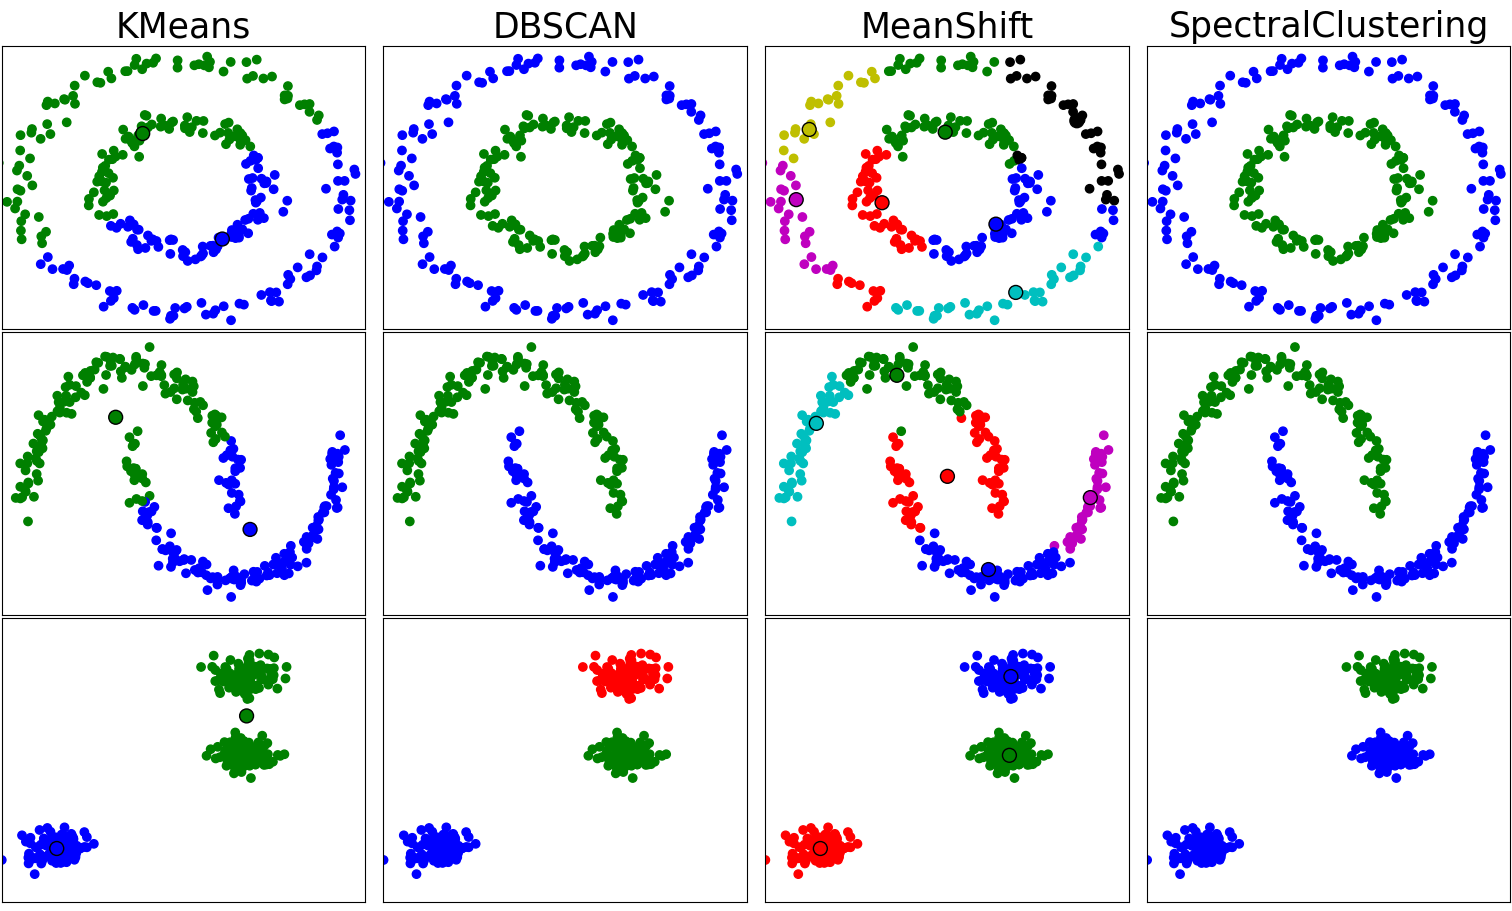
\includegraphics[width=\linewidth]{../files/DMS/images/classical_clustering_examples_2.png}
        \caption{Examples of classical clustering approaches. In cases where the method predicts cluster centres, these are shown with an outlined circle.}
    \label{fig__DMS__classical_clustering_examples}
 \end{figure} 

\subsection{Formulation}
Clustering algorithms aim to group a set of $n$ $d$ dimensional points $\{\mathbf{x}_1, \mathbf{x}_2, ..., \mathbf{x}_n\} = \mathcal{X}$ into $k \leq n$ sets $\{S_1, S_2, ... S_k\} = \mathcal{S}$ with centres $\{\boldsymbol{\mu}_1, \boldsymbol{\mu}_2, ..., \boldsymbol{\mu}_k\} = \mathcal{M}$. 

\begin{equation}
    \boldsymbol{\mu}_i = {\frac {1}{|S_{i}|}}\sum _{\mathbf {x} \in S_{i}}\mathbf {x}
\end{equation}
\myequations{Cluster Center Definition}
where $|S_{i}|$ is the number of points in cluster $i$.



\subsection{K-means}
The objective of k-means clustering is to divide a set of $n$ observations into $k$ clusters, with each observation being assigned to the cluster whose mean, often referred to as the cluster centre, is closest to it. This cluster centre acts as a representative of the cluster itself. The primary aim of k-means clustering is to minimise the intra-cluster variance, measured using L$_2$ distance, which consequently divides the data space into Voronoi cells. 
Mathematically:
\begin{equation}
    \argmin_{\mathbf{S}}\sum _{i=1}^{k}\sum _{\mathbf {x} \in S_{i}}\left\|\mathbf {x} -{\boldsymbol {\mu }}_{i}\right\|^{2}.
\end{equation}
\myequations{K-Means Optimisation Criteria}
\begin{algorithm}
\caption{k-means algorithm}\label{alg__DMS__kmeans}
\begin{algorithmic}
\Function{k-means}{$\mathcal{X}$, k}
\State Select $\{\boldsymbol{\bar{\mu}}^{(0)}_1, \boldsymbol{\bar{\mu}}^{(0)}_2, ..., \boldsymbol{\bar{\mu}}^{(0)}_k\} = \mathbf{\bar{\mathcal{M}}}$ a set of cluster centre initial estimates

\While{$\mathcal{S}^{(n)} \neq \mathcal{S}^{(n-1)}$}
    
    \State Assign each data point to the cluster with the nearest centre:
    
    \State $ S_{i}^{(n)}=\left\{x_{p}:\left\|x_{p}-\mu_{i}^{(t)}\right\|^{2}\leq \left\|x_{p}-\mu_{j}^{(t)}\right\|^{2}\ \forall p,  \forall j, 1\leq p\leq n, 1\leq j\leq k\right\}$
    
    \State Recalculate centres using the data points assigned to each cluste:
    
    \State $\boldsymbol{\mu}_i^{(n+1)} = {\frac {1}{\left|S_{i}^{(n)}\right|}}\sum _{\mathbf {x} \in S_{i}^{n}}\mathbf {x}$
\EndWhile
\EndFunction
\end{algorithmic}
\end{algorithm}
K-means and other similar algorithms are effective in cases where the number of clusters is known and the intra-cluster variation is lower than the inter-cluster variation. 
This is because they maximise the similarity of data points in the same cluster and maximise the difference between points in different clusters. However, this makes it unsuitable for cases where the clusters vary significantly in shape, size, or density. K-means is also very sensitive to the initialisation of the estimated means; see \Cref{fig__DMS__classical_clustering_examples} for examples of failure cases of k-means, where $k$ was not correct or the manifold of the data was such that there was greater intra-class than inter-class variation.

K-means++ \cite{Arthur2007} improves the cluster centre initialisation by finding spread-out sample points. K points are randomly selected as before, but they are selected sequentially, and the selection of a given point is weighted based on the reciprocal of the squared distance between it and other already sampled points. Another improvement on k-means was developed by \citet{xing2002distance}, who focused on learning a more appropriate distance metric using pairwise side-information. This idea has since been extensively explored \cite{Ceccarelli2008,ailon2018approximate,choudhury2019top,kim2017relaxed,mazumdar2017clustering} and motivated our work in \Cref{sec__DMS}.
K-means and its variants are useful because they are simple and robust. However, in practice, $k$ is often unknown. 

\subsection{DBSCAN}
Another branch of spatial methods is linkage methods. Linkage methods adopt a bottom-up strategy in which small clusters are merged using local neighbour criteria rather than information about the whole manifold. Examples are Ward's hierarchical clustering (AC-W) \cite{Murtagh2014} and DBSCAN \cite{Sander1998}. 

DBSCAN is a density-based clustering method that uses a maximum distance threshold, $\epsilon$, and a minimum neighbours threshold, $minPts$, to define its clusters.
DBSCAN initially generates a graph of points. Points are connected iff the distance between them is below $\epsilon$. 
Points are classified as core points, non-core points, and outlier points. Core points are directly connected to more than $minPts$ numbers of points. A cluster is defined by a graph that includes all directly connected core points and all non-core points that are directly connected to one or more core points. Outlier points are points not connected to a cluster, \ie any point that is neither a core point nor directly connected to a core point.

    









    




\begin{algorithm}
\caption{An abstract description of DBSCAN}\label{alg__DMS__dbscan}

\begin{algorithmic}
\Function{DBSCAN}{$\mathcal{X}$, $\epsilon$, minPts}
\State i = 0
\State $\mathbf{\mathcal{S}} = \{\}$
\ForEach{unvisited point $\mathbf{x} \in \mathbf{\mathcal{X}}$}
    \State mark $\mathbf{x}$ as visited
    \State $\mathbf{\mathcal{N}}$ = regionQuery($\mathbf{x}$, $\epsilon$), find the set of neighbouring points
    \If{$|\mathbf{\mathcal{N}}|$ $\geq$ minPts}
        \State $\mathbf{\mathcal{S}}_i = \{\mathbf{x} ,\}$
        \State $\mathbf{\mathcal{S}} = \mathcal{S} \cup \{\mathbf{\mathcal{S}}_i\}$
        \State expandCluster($\mathbf{x}$, $\mathbf{\mathcal{N}}$, $\mathbf{\mathcal{S}}_i$, $\epsilon$, minPts)
        \State i++

    \Else
        \State mark $\mathbf{x}$ as NOISE
    \EndIf
\EndFor
\EndFunction
\item[]
\Function{expandCluster}{$\mathbf{x}$, $\mathbf{\mathcal{N}}$, $\mathbf{\mathcal{S}_i}$, $\epsilon$, minPts}

\ForEach{point $\mathbf{x}' \in $ $\mathbf{\mathcal{N}}$}
    \If{ $\mathbf{x}'$ is not visited}
    \State mark $\mathbf{x}'$ as visited
    \State $\mathbf{\mathcal{N}}$' = regionQuery($\mathbf{x}'$, $\epsilon$)
        \If{$|\mathbf{\mathcal{N}}$'| $\geq$ minPts}
            \State $\mathbf{\mathcal{N}}$ $=$ $\mathbf{\mathcal{N}}$ $\cup$ $\mathbf{\mathcal{N}}$'
        \EndIf
    \EndIf
    \If{$\mathbf{x}'$ is not yet member of any cluster}
    \State $\mathbf{\mathcal{S}}_i = \mathbf{\mathcal{S}}_i \cup \mathbf{x}'$
    \EndIf
\EndFor
\EndFunction
\item[]
\Function{regionQuery}{$\mathbf{x}$, $\epsilon$}
\State return all points within $\mathbf{x}$'s $\epsilon$-neighborhood (including $\mathbf{x}$):
\State $\mathbf{\mathcal{N}} = \{\mathbf{y}| \mathbf{y} \in \mathbf{\mathcal{X}} \land ||\mathbf{y} - \mathbf{x}||_2 \leq \epsilon\}$  
 
\EndFunction

\end{algorithmic}
\end{algorithm}




If the number of clusters and the minimum cluster size are known, then a search over $\epsilon$ can be used to find the appropriate clusters.

As DBSCAN and other similar linkage-based methods only look at local neighbourhood densities rather than using a broader dataset-wide viewpoint, they show good performance in cases when the shape of the clusters varies significantly.
They also often work well in cases where there are outlier points or noise since unlike methods like k-means, they are not required to assign all points to a cluster. 
DBSCAN significantly differs from k-means as it can create clusterings where some intra-cluster distances exceed some inter-cluster distances by an arbitrary amount; see \Cref{fig__DMS__classical_clustering_examples}.

The performance of DBSCAN and other linkage-based methods are significantly degraded in higher dimensional feature spaces as their affinity measures are grounded in observations of low-dimensional data \cite{ertoz2003finding}.
GDL \cite{Zhang2012} works in a similar fashion to DBSCAN but defines a more complex affinity metric using the average in-degree and out-degree of each data point. 
This makes it more robust to noise, and it proves more consistent in high-dimensional feature spaces. 


\subsection{Mean shift}\label{sec__litreview__meanshift}
Mean shift is a non-parametric `mode-seeking algorithm'. In its simplest form, it iteratively locates an estimate of the maxima of a density function given discrete samples from that function. 
An estimate for the maxima is found by taking a previous estimate and a weighted average of points proximal to the previous estimate. The weights for the average are typically based on the distance from the current estimate using a Gaussian Kernel. The vector between one estimate and the next is called the \textit{mean shift} \cite{Fukunaga1975}. This process is repeated until the algorithm has converged. There is currently no formal proof for the convergence of mean shift in high (>1) dimensional space using a general kernel \cite{ghassabeh2015sufficient}.

In a clustering context, mean shift iteratively improves its estimate of the cluster's centre or sample mean by averaging the position of points it currently believes are inliers to that cluster. Data points that converge to the same sample mean are grouped together into a single cluster.
In order to sort a whole dataset, the classical mean shift algorithm must be initialised from each data point.

Classical mean shift is based on two key assumptions: firstly, points that are similar belong to the same cluster, and, secondly, that Euclidean distance is a good proxy for similarity.

The mean shift algorithm is formulated as follows.
Given a set of data points, $\mathcal X$, an estimate of the cluster centre $\bar{\boldsymbol{\mu}}^{(n)}_i$ associated to point $\mathbf{x}_i$ is improved using the sample mean function $m$ as:

\begin{equation}\label{eq__DMS__mean_shift}
    \bar {\boldsymbol{\mu}}^{(n+1)}_i = m(\mathcal{X}, \bar {\boldsymbol{\mu}}^{(n)}_i) = \frac{\sum_{\mathbf x \in \mathcal X} \mathbf x K(\mathbf x, \bar {\boldsymbol{\mu}}^{(n)}_i) }{\sum_{\mathbf x \in \mathcal X} K(\mathbf x, \bar{\boldsymbol{\mu}}^{(n)}_i)},
\end{equation}
\myequations{Mean-Shift Iteration}
where $K(.)$ is a kernel function which evaluates the similarity of two $n$ dimensional points in a 0 to 1, dissimilar to similar, range.

Given the sample mean function $m(.)$ defined on some collection of data with an initial value $\bar{\boldsymbol{\mu}}^{(0)}$, a cluster centre together with the cluster inlier data points can be calculated using the mean shift algorithm. The sample mean is iteratively updated until the distance of sample means between two consecutive iterations becomes sufficiently small, \ie $\|\bar{\boldsymbol{\mu}}^{(n+1)} - \bar{\boldsymbol{\mu}}^{(n)} \| < \tau_c $, where $\tau_c$ is the convergence threshold; see \Cref{alg__DMS__meanshift}. The difference between an estimate of the sample mean $\bar{\boldsymbol{\mu}}^{(n)}$ and the initial estimate of the sample mean, $\bar{\boldsymbol{\mu}}^{(n)}- \bar{\boldsymbol{\mu}}^{(0)}$  is known as the \textit{total mean shift}. 

\begin{algorithm}
\caption{Mean-Shift Algorithm}\label{alg__DMS__meanshift}
\begin{algorithmic}
\Function{Mean-Shift}{$\mathcal{X}$, $\tau_c$}
\State Initialise a set of centre estimates $\{\boldsymbol{\bar{\mu}}^{(0)}_1, \boldsymbol{\bar{\mu}}^{(0)}_2, ..., \boldsymbol{\bar{\mu}}^{(0)}_k\} = \mathbf{\bar{\mathcal{M}}}$

\ForEach{$\boldsymbol{\bar{\mu}}^{(0)}_i \in \mathbf{\bar{\mathcal{M}}}$}

    \While{$\left\|\bar {\boldsymbol{\mu}}^{(n)}_i - \bar {\boldsymbol{\mu}}^{(n-1)}_i\right\| \geq \tau_c $}
        \State 
         $
            \bar {\boldsymbol{\mu}}^{(n+1)}_i = m(\mathcal{X}, \bar {\boldsymbol{\mu}}^{(n)}_i) 
        $
        
    \EndWhile
\EndFor
\EndFunction
\end{algorithmic}
\end{algorithm}

To cluster all points, the algorithm must be initialised from each point $\bar{\boldsymbol{\mu}_i}^{(0)} = x_i $ for all $x_i \in \mathcal{X}$ (i.\ e.\ $k=n$). The data points are then grouped based on their estimated centres after convergence, \ie if $\left\|\bar{\boldsymbol{\mu}_i} - \bar{\boldsymbol{\mu}_j}\right\| < \tau_s$,
then $x_i$ and $x_j$ are in the same cluster, $S = \{i, ... , j, ...\}$.

Mean shift can also be used on a subset of points to find centres which then act as initialisation points for another clustering method such as k-means.
In \Cref{sec__DMS}, we present a method inspired by the iterative approach of cluster finding used in mean-shift. 
Our method, however, uses a neural-network-based similarity kernel which allows it both to work more effectively in high-dimensional feature spaces and to address different tasks more flexibly.

\subsection{Spectral clustering methods} 
Spectral clustering methods \cite{VonLuxburg2007, Nie2011, Shi, Ng2002, shi2003multiclass} aim to reduce the dimensionality of a feature space before clustering it using any of the above methods.
This is achieved by converting an $n\times n$ data point distance graph into its Laplacian and taking the $k$ most significant eigenvectors to form a $n\times k$ \textit{spectral embedding}; see \Cref{alg__DMS__spectralclustering}. This spectral embedding can be used to improve the performance of other clustering methods, such as k-means. 

\begin{algorithm}
\caption{An abstract description of Spectral Clustering}\label{alg__DMS__spectralclustering}
\begin{algorithmic}
\State Generate a similarity matrix $\mathbf{A}$ of all points, $\mathbf{A}_{ij}\geq 0$

    \State Calculate the Laplacian $\mathbf{L}$ (or the normalised Laplacian)
    $\mathbf{L}=\mathbf{D}-\mathbf{A}$ where $\mathbf{D}$ is the diagonal matrix $\mathbf{D}_{ii}=\sum _{j}\mathbf{A}_{ij}$
    
    \State Compute the eigenvectors associated with the $k$ least eigenvalues of matrix $\mathbf{L}$
    
    \State Construct the spectral embedding, the $n \times k$ matrix taken from the first $k$ eigenvectors


    \State Cluster the n graph nodes in this new spectral feature space

\end{algorithmic}
\end{algorithm}

As spectral clustering methods decrease the dimensionality of the data, they handle cases with high-dimensionality or non-standard manifolds well. However, their performance in cases with outliers or noise is significantly reduced as the eigenvectors of the Laplacian are very sensitive to perturbations \cite{grady2006isoperimetric}.

\subsection{Deep Clustering}\label{sec__DMS__rel_deep}
Most classical clustering approaches use simple metric functions and work well with low-dimensional data. However, they generalise poorly to higher dimensions given the added complexity of finding affinity in higher-order feature spaces \cite{Aggarwal2001}. This phenomenon is closely related to the `curse of dimensionality' \cite{Domingos:2012:FUT:2347736.2347755, Bellman1962}. 

Prior deep learning methods attempt to either (i) encode data points into a features space that can be more effectively clustered using classical methods or (ii) mimic and improve upon conventional spatial/spectral clustering approaches with a set of differentiable layers
\cite{aljalbout2018clusteringtaxonomy}.

DCN \cite{Yang2017} trains a deep neural network to perform an optimised, non-linear dimensionality reduction and then uses k-means clustering. They train their dimensionality reduction stage using a k-means loss.
This enforces a condition that the assigned data points are evenly distributed around the cluster centres.
Jule \cite{Yang2016} uses an agglomerative clustering loss to find an appropriate and reduced feature space. Jule uses an iterative approach where data points are clustered based on an affinity metric.
Their network is then trained to further optimise the affinity in the now-merged clusters. This process repeats, resulting in a feature space best optimised for hierarchical methods like agglomerative clustering or DBSCAN. 

Deep Embedding for Clustering (DEC) \cite{Xie2016} and DEPICT \cite{Dizaji2017} use a combination of an autoencoder-reconstruction loss to reduce the dimensionality of the feature space and a cluster-assignment loss. The cluster-assignment losses aim to make soft cluster predictions align with a set of target predictions, pushing points deemed similar closer together in the lower dimensional feature space.
Similarly, DAC \cite{Chang2017} creates a feature space which it iteratively improves by driving similar points together using a binary pairwise classification loss.


While linear projections and autoencoders are the most commonly used dimensionality reduction approaches, other methods have been proposed to similar effect. \citet{Hu2017},  \citet{Hsu2018}, and \citet{VittalPremachandran2017} utilise either self-augmentation or Generative Adversarial Networks (GANs) to reduce the dimensionality of their respective feature spaces while maintaining or improving the understanding of data point similarity.
The impact of these improved feature spaces is clear.

Most of the above methods boast significant improvements on high-dimensional data as compared to the classical methods upon which they are based.
However, these methods generally focus solely on improving the suitableness of the feature space for classical clustering rather than changing the method of clustering itself.

Deep clustering approaches that are based on classical clustering methods generally have the same flaws as those classical methods such as requiring supervision in the form of dataset-specific parameters. This parameter-tuning significantly decreases the usefulness of these clustering approaches in applications where end-to-end training is required as well as in deployment contexts where users may not have the knowledge needed to tune these parameters.

Robust Continuous Clustering (RCC) \cite{Shah2018} and Deep Continuous Clustering (DCC) \cite{shah2018deep} both create an improved feature embedding and then generate the clusters directly. They use a locality-preserving loss to learn a more robust feature embedding that is consistent with a classical $k$-NN graph, bringing mutual $k$-NN samples closer to create tighter clusters. 
\citet{Shah2018} also proposed RCC-DR which utilises a linear autoencoder for dimensionality reduction.
Instead of using a classical clustering method on the embedded feature space to generate discrete cluster definitions, both RCC and DCC generate clusters in a continuous fashion. This allows them to be more easily incorporated into methods trained in an end-to-end fashion.

In \Cref{sec__DMS}, we focus on clustering a feature space without explicitly embedding it. This is because it is not always possible or efficient to train an encoder for the clustering stage, such as when the clustering is added as a head to a system that is required to be memory and time-efficient. 
While many methods need fully-labelled training data, we do not wish to impose this requirement as it would severely limit the viable deployment scenarios of our method.
While the work presented in \Cref{sec__DMS} focuses explicitly on clustering difficult-to-divide datasets using simple untrained features, the above encoding methods could be complimentary as they would likely improve the input feature space making clustering simpler. 

\subsection{Side-Information}
Completely unsupervised methods, although highly appealing as they do not require the laborious labelling of data, cannot exploit externally applied semantic concepts.
This can result in learned representations that prove challenging to interpret and may not align with a user's understanding.
Side-information based approaches aim to strike a middle ground, allowing a user to align the learned insights to their knowledge of the data but not requiring large-scale data labelling.
Side-information generally refers to information known about the data that cannot be directly used to supervise training, \ie it is not the ground truth label.
Pairwise co-cluster labelling as introduced by \citet{xing2002distance} is a good example of side-informational supervision. 
Pairwise labels define a list of pairs of data points that are `similar' and a list of pairs that are `dissimilar'  without labelling any other information. These pairwise relational labels are, in many cases, easier to gather than more descriptive labels like the ground-truth class of a data point.
Pairwise information can be used to find, or act as a substitute for, other required information such as a distance tolerance. 

Pairwise labels are commonly utilised in two separate ways, Metric Learning \cite{bar2005learning, bilenko2004integrating, chang2004locally, xing2002distance} and Constrained Clustering \cite{shental2003computing, lu2004semi}. In the former, a feature space is learnt prior to clustering which minimises the intra-cluster variance of similar points while maximising the inter-cluster variance of dissimilar points. 
In the latter, the clustering algorithm itself is altered to penalise grouping dissimilar points and not grouping similar points.

Deep-learning-based clustering methods that use pairwise side-information also follow these two paradigms.
\citet{Hsu2015} use a neural network to predict a cluster membership probability vector for each data point which is then evaluated using a constrained clustering loss.
The pairwise supervision is then used in combination with a contrastive KL-divergence term to penalise similar pairs having different cluster membership probabilities and dissimilar pairs having similar cluster membership probabilities.
\citet{Fogel2019} improves upon RCC \cite{Shah2018} by using pairwise constraints to strengthen or remove the links between data points found using K-NN. 
They utilise a Siamese autoencoder network to generate representations of pairs of data points. 
They then use a clustering loss in combination with a reconstruction loss to encourage diverse and meaningful latent representations which are proximal for similar pairs and distant for dissimilar pairs.
\citet{shukla2020semi} is similar to \citet{Fogel2019} in that they train a convolution autoencoder with a combination of a metric learning loss term and a reconstruction loss. It encodes latent representations suitable for k-means clustering, encouraging low intra-cluster variance, while simultaneously regressing cluster centres.
They also incorporate a cluster membership KL divergence term as in \citet{Hsu2015}.
Various works have looked into the resilience of clustering methods to errors in pairwise supervision \cite{Mazumdar2017,choudhury2019top} as well as into how they are affected by having non-binary `similar'/`dissimilar' boundaries \cite{kim2017relaxed}.

As our clustering method, presented in \Cref{sec__DMS}, must be lightweight, it does not employ the metric learning approaches of many other methods and instead takes a constrained clustering approach. The metric learning stages are generally used prior to a clustering stage which uses a classical distance metric and so do not scale well to high-dimensional spaces. Instead, our method learns a minimal, but high-dimensional, kernel which can estimate the similarity of data points, in the original high-dimensional feature space.

\section{Counting}
As mentioned in \Cref{sec__intro__objective}, we believe counting is comprised of two processes: identifying objects that could be of interest and enumerating the repetitions of them. The latter process can be approached as clustering.
In the established literature, \textit{`Counting'} is used to describe systems which include both the instance finding stage as well as the clustering or repetition recognition stage.
Most commonly, automated counting is applied in the context of computer vision and image processing, though it could in theory be applied to other data modalities.

\subsection{Class-specific counting}
Generally, methods that have aimed to complete the whole task of counting, that is finding and enumerating objects, have focused on counting a single or small set of known classes of objects.
These class-specific counters have been useful in a variety of industries, including ecology with animal counting \cite{go2021fine, arteta2016counting}, urban planning with vehicle \cite{arteta2014interactive, Lu18, mundhenk2016large} and crowd counting \cite{wang2011automatic, wang2015deep, marana1997estimation, cao2018scale, barinova2012detection, Lu18}, and various medical and biological disciplines that require cell counting \cite{xie2018microscopy, morelli2021automating}. 
These industries all benefit from being able to gather accurate and reliable data in a short amount of time with minimal manual labour.

Class-specific methods are trained to locate a specific type of object. They require an individually trained network for each type of object to be counted, with limited to no capacity to adapt to novel classes.
Individually trained networks require gathering new data and retraining whenever a new type is considered, which is difficult, time-consuming, and expensive.  
Additionally, these methods generally aim to explicitly localise instances before enumerating them, requiring point-level annotations to supervise the training. 
These class-specific and point-level supervised systems are only feasible when the composition and appearance of object types will remain the same indefinitely and point-level annotations exist, which is often not the case in real-world applications. 
Counting methods can be broadly grouped into detection-based, regression-based, and classification-based methods.

\subsection{Detection-based Counting} 
Detection-based methods use standard object detection or segmentation approaches \cite{ren2015fasterrcnn, michaelis2018one} to find all objects of a given type and then enumerate them.  This can be used on either a single class \cite{hsieh2017drone} or on multiple classes \cite{desai2011discriminative}. 
Detections can be found using the original input image or a constructed feature space such as local-maxima detection on a regressed density map \cite{liang2022focal, barinova2012detection, arteta2014interactive, cholakkal2020towards, xu2022autoscale}. 
Detection-based methods are often trained using bounding box labels which are more expensive to gather than the point- or image-level annotations used by some other branches of methods.
To bridge this gap, some methods aim to use topological information to improve their results when only using point annotations \cite{abousamra2021localization, liu2019point, liang2022focal, xu2022autoscale}. 
For example, \citet{liu2019point} generate pseudo-ground truth bounding boxes from their point-level annotations, and \citet{abousamra2021localization} combine density map regression with a detection stage which learns topological information about the probability that people are near each other and uses this to inform more accurate predictions.
These methods, however,  generally have worse performance than those that use full bounding box supervision. 

Detection-based methods work best in settings where individual objects are easily distinguishable.
Object detection and segmentation, separate from counting applications, are broad fields with significant recent developments that can be beneficial in counting applications. Their performance in cases with high overlap or occlusion has improved materially in recent years. However, detection-based counting methods are still unsatisfactory in high-density applications, applications with complex or highly textured objects,  or applications with large intra-class variation and low inter-class variation.


\subsection{Classification-based Counting}
Classification-based methods \cite{mundhenk2016large, Aggarwal2001} generate a discrete classification of an image's global count. 
Their most obvious flaw is that they treat each `count class' independently rather than as a continuous variable. 
This means all incorrect counts, independent of their proximity to the ground-truth count, are treated as equally wrong. 
This makes training difficult as you need data from each discrete count-class, meaning you either need large amounts of data and/or a low maximum count.
\citet{8846229} partially solved this by using a nonlinear quantisation strategy and making block-wise classifications to generate a `coarse count level' rather than the exact count for areas of an image. This produced a fairly accurate classification counter. However, it was imprecise, generating only a range that the count fell into, not the exact value.

\subsection{Regression-based Counting} 
Regression-based counting methods aim to regress a single image-wise count \cite{chan2009bayesian, wang2011automatic, wang2015deep} or a pixel-wise density map prediction \cite{lempitsky2010learning, cao2018scale, ranjan2021Famnet, xie2018microscopy}.
The pixel-wise density map prediction is such that when an area is integrated, it gives a count value for the corresponding area of the image.

Regression methods that aim to find density maps are often cheaper to train than detection-based approaches as they only require point annotations rather than bounding boxes. 
Point annotations already exist for datasets in many fields as the process of `dotting' or `pointing' is standard practice for manual counting \cite{8578940, zhang2016single, sindagi2020jhu, cohen2017countception, 10.1007/978-3-319-24574-4_33, Gao_2021}.
The approximate ground-truth density map is then generated by placing a Gaussian kernel centred at each point annotation.

Density map regression methods have been around for a long time \cite{marana1997estimation} and operate in various ways using features ranging from simpler low-level classical features \cite{chan2009bayesian} such as texture \cite{marana1997estimation, 757602, marana1998automatic} to complex features generated from neural networks  \cite{zhang2015cross,zhang2016single}. 
As regression-based methods generate a decimal count rather than a definite integer, they were originally only used to estimate the overall count in cases where the objects were hard to detect individually. However, recent methods are more precise and can better locate specific instances in complex settings rather than estimating the density of the instances.
A regressed density map can also be used as a rudimentary object detector, followed by cross-correlation with an exemplar to find instances of the desired class, such as in \citet{sokhandan2020few}.

While density map regression-based methods can produce accurate counts, they are often blurry and cannot accurately locate individual instances in dense environments \cite{cholakkal2020towards, xu2022autoscale} due to their use of a Gaussian kernel for ground truth generation.

In this thesis, we approach counting as a regression task. We show that for single-class images, as posed in most of the prior literature, density map regression is not needed and that scalar image-wise count regression is sufficient. We then go on to show that in more complex, multi-class images, density map regression is useful for disambiguating counts during training and for quantitative analysis.
 
\subsection{Weakly-supervised Counting} 
The majority of the counting methods outlined above use some form of instance-wise positional information, which is costly to gather. 
Weakly-supervised counting methods aim to generate an accurate count with a reduced annotation burden. They are trained with minimal \cite{lei2021towards, sam2019almost} or no point-level annotations \cite{borstel2016gaussian, yang2020weakly, wang2015deep}.
The methods to facilitate training of an accurate model with reduced supervision vary greatly.

\citet{borstel2016gaussian} proposed the use of Multiple Instance Regression (MIR) to reduce the normal labelling requirements. This formulation uses a set of annotated counts corresponding to regions of the image. The exact location of the instances is not labelled. The model then learns to assign pixel-level densities to match the region-level counts.

MATT \cite{lei2021towards} is trained predominantly using count-level annotations but with a small amount of point-level annotations. They found that training a single network with a single count value was not sufficient in constraining their problem. Instead, they found that training multiple networks which all have to generate the same count given the same input added a coherence constraint sufficient to make their results competitive.

\citet{yang2020weakly} proposed a soft-label sorting network that is trained mostly by trying to sort images by count. They found this helped them generate more representative features that were then used to directly regress the image-wise count.

Another approach to minimising the annotation burden is to conduct most of the training in an unsupervised way.
\citet{sam2019almost} took this approach, optimising 99.9\% of their stacked auteoencoders' parameters with unlabelled data. The remaining 0.1\% of parameters were optimised using point-level annotations. 

\citet{liu2018leveraging} use a self-supervised approach to gain a meaningful understanding of counting by utilising completely unlabelled crowd data during training. They do this by creating a ranking network that orders a set of hierarchical crops from a crowd image. This is built on the fact that a cropped version of an image must have an equal or lower associated count than the uncropped image. 
This proxy task, which uses easy-to-gather unlabelled images, improved their accuracy by an average of 10\%.

We endeavour, where possible, to minimise the amount of labelled training data required to learn to accurately count.
To this end, we show in \Cref{sec__LTCA} that in settings with only a single kind of object present and so with minimal ambiguity, weak supervision is all that is needed to learn to count, even when the kind of object is novel.


\subsection{Class-agnostic Counting}
In contrast to the class-specific methods above, which require a static class composition, class-agnostic counting methods, introduced in 2018 \cite{Lu18}, aim to learn a general understanding of counting that can be applied to arbitrary classes. 
This means they can, in theory, count objects of types they did not encounter during training, which makes them useful for deployment in many more fields, where gathering large amounts of data may be prohibitively expensive or time-consuming.
In general, class-agnostic counting has been achieved by creating a sufficiently general feature space and then applying some form of matching to the whole feature map \cite{yang2021cfoc, shi2022represent} or to proposed regions of interest \cite{ranjan2021Famnet, sokhandan2020few}.
This matching utilises an exemplar image, which is provided at both training and inference time, to serve as an example of the type of object to be counted.

The first class-agnostic counting method, Generic Matching Network (GMN) \cite{Lu2018}, introduced the idea of performing counting in an extract-then-match way.
They had a very simple approach to this.
They embed the exemplar and query images into the same feature space, concatenate them, and then match them using an architecture comprised of a (3 $\times$ 3) convolutional layer and a (3 $\times$ 3) convolutional transpose layer in order to generate a density map of the same resolution as the input image.
They utilised tracking video data to train a backbone with a general feature space which they then fine-tuned to specific domains using labelled data on the order of dozens to hundreds of images.
GMN struggles with completely novel classes without fine-tuning \cite{ranjan2021Famnet}.

\citet{ranjan2021Famnet} improved upon the class-agnostic paradigm laid out by \citet{Lu2018} with FamNet, which can achieve counting on previously unseen classes without the need for domain-specific adaptation. 
They achieve this using a multi-scale feature extraction module, which generates meaningful general features, and a density prediction module, which matches features and regresses a density map.
They achieve multi-scale feature matching by performing ROI pooling on the convolutional feature maps from sequential blocks from their pre-trained backbone that are at different resolutions.
\citet{ranjan2021Famnet} also incorporated two test-time adaptations to improve their results, both of which were based on the exemplar images being drawn from the query image. They firstly apply a scaling based on the knowledge that the exemplar bounding box must contain $\geq$1 instance. Secondly, they apply an idea similar to correlation filters which are used in in tracking \cite{henriques2014high}.
The idea is that as perturbations to the bounding box increase, the target response should decrease, in this case following a Gaussian distribution.
These two adaptations are combined and applied as a loss at test time to simulate a single-query fine-tuning.

\citet{shi2022represent} expand upon the extract-then-match paradigm of previous methods with BMNet and BMNet+, which learns a similarity metric and loss jointly with the feature representation. Their learnt similarity loss is inspired by metric learning \cite{schultz2003learning}, specifically that a good similarity metric should be low for features drawn from different categories and high for features drawn from the same category. 

At the point of conducting the work in \Cref{sec__LTCA}, there were no exemplar-free counting methods, and all class-agnostic counting methods utilised instance-wise annotations, \ie there were no weakly-supervised class-agnostic counters.
We believe that such a method is possible and desirable for three reasons.
First, given the human ability to arbitrarily count objects, 
why should algorithmic counting methods need exemplar images?
Second, removing the need for exemplar images increases the deployment utility of our method as human intervention is no longer needed.
Third, given the success of weakly-supervised class-specific counting methods, the requirement of instance-wise locational annotations in class-agnostic counting is unnecessary.
In \Cref{sec__LTCA}, we show all of this to be the case. 
That is, a weakly-supervised exemplar-free class-agnostic counting method is not only possible but competitive with exemplar-based and strongly-superverised contemporary methods in single-class settings.


It should be noted that class-agnostic counting is distinct from multi-class counting, where objects of different classes appear within the same image. Before our work, class-agnostic counting had only been approached in single-class settings. 
\citet{Lu18} qualitatively demonstrated their abilities on images with a single class of object present and quantitatively evaluated their method on cell microscopy images \cite{arteta2016detecting, lempitsky2010learning, lehmussola2007computational} and drone-collected car images \cite{hsieh2017drone}, all of which only have one kind of object present. 

Following its introduction in 2021 \cite{ranjan2021Famnet},  FSC-147 has become the default class-agnostic counting dataset \cite{ranjan2021Famnet, ranjan2022exemplar, liu2022countr, shi2022represent, lin2021object}.
Almost all of the images in FSC-147 contain only a single type of object, and in the few cases with multiple object types, only one is labelled.
This has created a situation where class-agnostic counting methods are incentivised to develop an understanding of counting which is based on the idea of `generic object detection' rather than having a discriminative approach which only counts similar objects.

While some exemplar-based methods were assumed to have the ability to function robustly in settings with more than one class of object present this has not been proven. In fact, we found this not to be the case; see \Cref{sec__ABC123} for details. Our work, detailed in \Cref{sec__LTCA}, shows that a method with no class-direction (\ie no exemplar images) can achieve state-of-the-art results on FSC-147, demonstrating that it contains few images in which it is ambiguous what is to be counted.

As it is clear that a good dataset encourages the development of methods to address it, and it is of course useful to have tools that function in multi-class settings, we created the first multi-class class-agnostic counting dataset, presented in \Cref{sec__MCAC}.
We utilise this dataset in the development of the first multi-class exemplar-free class-agnostic counting method, detailed in \Cref{sec__ABC123}. 
Unlike existing methods, this method simultaneously counts objects of multiple classes and is robustly shown to differentiate between different classes rather than functioning as a generic object detector.


\subsection{Attention in Counting}
Inspired by the success of attention-based architectures and transformers in other tasks, various methods aim to utilise these advancements in counting.
\citet{liu2019adcrowdnet} propose the Attention Map Generate (AMG) which generates two priors for a CNN, a mask of important `candidate' regions and a `congestion degree' which estimates a range of likely count values. The former aids the following stages in focusing on areas of high importance, for example, ignoring noisy backgrounds. The latter allows the later stages to generate more precise answers by focusing it on a smaller range of possible values.

\citet{jiang2020attention} works in a similar way, proposing regions of interest with a Density Attention Network (DANet) and then using an Attention Scaling Network (ASNet) to correct for systemic under- and overestimating errors. This method multiplies the counts by an attention score, effectively generating different counts for different areas and then summing them.
\citet{zhang2019attentional} proposed the Relation Attention Network (RANet) which utilises local and global self-attention on CNN features. This creates more informative features which can capture dependencies over the whole image. 


In 2021, \citet{liang2021transcrowd} proposed CLTR, the first method to apply transformers to crowd counting with limited or no point-wise labelling, \ie weakly-supervised crowd counting.
This was followed by various other crowd-counting methods including CrowdFormer \cite{savner2022crowdformer}, JCTNet \cite{wang2022joint}, and TDCrowd \cite{do2021attention}.
CrowdFormer \cite{savner2022crowdformer} is a transformer-based method which addresses issues of people appearing at varying scales in a single image. 
It utilises a pyramid-structured vision transformer to capture multi-scale information. This is similar to many multi-scale  CNN methods, but it incorporates the global receptive field of a transformer.

\citet{wang2022joint} recognised that patching images during counting tasks can cause significant issues. If an object spans a patch boundary, it could be counted in both or neither, causing erroneous results. 
Their method, JCTNet, combats this issue by utilising the fact that convolutional network features are locally aware. They use convolutional layers to create locally aware features which are then passed to a transformer architecture to perform the final counting. This significantly improves their results when objects spanned patch boundaries.

TDCrowd \cite{do2021attention} is similar to the above methods in that it can be trained in a weakly-supervised pipeline, but it can also be trained with point-level labels. When trained with weak-supervision it achieved similar results to CLTR \cite{liang2021transcrowd}. However, when it is trained with instance labels, it is  $\sim$15\% more accurate, showing that even with a more contextually aware backbone, locational supervision is beneficial to counting tasks.

All of the above attention-based methods focus on crowd-counting, a class-specific task with limited ability to generalise to class-agnostic contexts.
Lao-net \cite{lin2021object} was the first method to use attention in a class-agnostic setting. It utilises a feature correlation module which is composed of Self-Attention and Correlative-Attention modules to learn inner-relations and inter-relations. The Self-Attention module creates more informative globally-aware features. The Correlative-Attention module then takes the place of the feature-matching convolution of most other class-agnostic counting methods. They achieve significantly better results ($\sim$35\% better MAE) than the prior, non-attention-based class-agnostic counting methods. However, they require both exemplar images and point-wise supervision.


In this thesis, we recognise the power of the vision transformer architecture and how it is uniquely suited to counting tasks. 
As such, we utilise it to its fullest.
In \Cref{sec__LTCA}, we show that the features generated from a well-trained vision transformer are sufficient to perform class-agnostic counting in single-class scenarios without exemplar images or instance-wise supervision.
In \Cref{sec__ABC123}, we expand on this, proposing an exemplar-free method which works in settings with multiple objects present, counting each simultaneously.



\subsection{Count Ambiguity}\label{sec__lit_rev__count_valid_but_unkonwon_counts}
Different counting tasks have significantly different levels of associated ambiguity.
Class-specific methods have very little ambiguity. The task is posed as `How many instances of type x are in the query image?'. 
As long as one can train a network to have a robust understanding of the complete variation of the desired type, this has no ambiguity. However, in settings without an expectation of visual coherence between the training and inference time images, this approach cannot be taken.

An exemplar-based class-agnostic counting method is easily understood and relatively unambiguous. The task is posed as `Given an exemplar image, how many of this type are present in this query image?'. 
In theory, a well-trained exemplar-based method can be applied to images with either a single type of object present or many kinds of object present. However, in \Cref{sec__ABC123}, we found that current exemplar-based methods \cite{ranjan2021Famnet,shi2022represent,liu2022countr} were not discriminative enough of object-type to achieve this robustly, mainly due to the available training data.
While this setting is usually well-defined, it is clear that the exemplar images will not capture the full distribution of the possible visual appearance of the objects. This introduces an ambiguity. An informed guess must be made on what is of the `same type' as the exemplars.
For example, given two exemplars of blue cars, should the network count all cars present in an image or just the blue ones?

In a known single-class exemplar-free setting, the question being posed is also relatively simple and unambiguous, `How many objects of the \textit{main} type appear in this image?'. 
While there is some ambiguity around `main', in single-class settings with only one kind of object, this is not an issue. This is shown in \Cref{sec__LTCA} where RCC achieves results on the FSC-147 dataset competitive with exemplar-based methods without the need for exemplar images.

In an exemplar-free setting with multiple types of objects, the objective is a lot less clear. 
When multiple types of objects are present and no guidance is given, there is an ambiguity of which count or counts are the desired output. 
An end user may want a single count, a specific set of counts, or all of the possible counts. 
There are also various ways to divide up a set of objects (size, colour, shape, semantic information) which would lead to multiple counts being associated with a single object.

To provide meaningful information to a user or to evaluate the accuracy of a method, it is important to be able to disambiguate the counts. This is achieved by either providing enough information to explain the count or by matching the predicted counts to the known class-count labels. This matching is non-trivial and likely not exclusive to those defined by the dataset creator. It is likely the data contains what we call \textit{valid-but-unknown counts}, which in turn the network will find.

Valid-but-unknown counts are associated with the ways of grouping objects differently from the known target labels.
They are likely to arise in any class-agnostic counting problem but are especially impactful in the context of  exemplar-free multi-class class-agnostic counting. 
There are many types of valid-but-unknown counts, for example: 
\begin{itemize}
    \item \textbf{Super-set counts}, it would be valid to count 4 dogs and 3 cats as 7 `animals'.
    \item \textbf{Sub-set counts}, 6 chess pieces could be counted as 2 white pieces and 4 black pieces.
    \item \textbf{Orthogonal-counts}, 2 red cars, 2 blue cars, 3 red boats and 3 blue bloats could be counted as 5 red objects and 5 blue objects or as 4 cars and 6 boats.
\end{itemize}

The idea of valid-but-unknown counts is closely related to our intrinsic and non-intrinsic task paradigm posed in \Cref{sec__DMS}.

\subsection{Conclusion}

This thesis was motivated by the mentioned prior work, their successes, and their limitations.
Prior clustering methods are often inflexible, requiring hyper-parameter tuning, large amounts of knowledge about the dataset as a whole, or only finding the intrinsic clusters.
In \Cref{sec__DMS}, we expand upon current clustering methods with DMS. 
DMS is a flexible and fully-differentiable clustering algorithm.
It utilises pairwise side-information to develop a task-specific understanding of similarity.

Prior to our work, counting methods required a static class composition or exemplar images during training and inference to define the type of object to be counted. Most of them also generally utilised point-wise instance labels.
In \Cref{sec__LTCA,,sec__ABC123}, we propose RCC and ABC123. RCC was the first exemplar-free class-agnostic counting method and the first weakly-supervised class-agnostic counting method. 
It not only demonstrates that counting objects of novel type without an exemplar is possible and that class-agnostic methods can be trained using only image-wise counts for supervision, but it also shows that they can be competitive with exemplar-based methods in single-class environments.

ABC123 is currently the only exemplar-free multi-class class-agnostic counting method. Unlike prior methods, it can generate counts for multiple novel types of objects simultaneously. 
\Cref{sec__ABC123} also introduces the idea of example finding. This paradigm turns the prior class-agnostic counting methods on their head. Instead of providing exemplars of the type to be counted, it performs exemplar-free counting and then generates examples of the types that have been counted.

In order to train and evaluate RCC and ABC123, we need robust and reliable datasets.
As discussed, FSC-147, the most popular class-agnostic counting dataset, only addresses single-class situations. 
It also contains errors.
As such, we present FSC-133 and MCAC in \Cref{sec__Datasets}.
FSC-133 is an updated version of FSC-147, which removes its errors and ambiguities. 
MCAC is the first multi-class class-agnostic counting dataset.

\end{document}